\subsection*{Step 2.3}

To determine the values of $a_i$ and $b_i$ for $i \in \{1,2,3,4\}$ that minimizes the squared area between $f$ and $\hat{f}$, a new PWA function of $f(u_d)-\hat{f}(u_d)$ has been created where the regions of $f(u_d)$ have been synced with the four functions of $\hat{f}(u_d)$. This created four separate minimization problems which have been minimized with \textit{fmincon()}. Equailty constraints were used, so that the functions have the same function value at the boundary. The steps to arrive at the given solutions are:
\begin{itemize}
    \item First approximate the first part, results in $a_1$ and $b_1$.
    \item Then, compute $\hat{f}(u_d)$ at the end of the first part (at $u_d$ = 5).
    \item Solve for the second part $(5\leq u_d<6.5)$ with an equality constraint $a_1+5b_1 = a_2+5b_2$.
    \item Repeat this for all parts.
\end{itemize}
A Matlab script \ref{} has been created to perform this PWA approximation, which can be examined for further explanation.

\begin{figure}[ht]
    \centering
    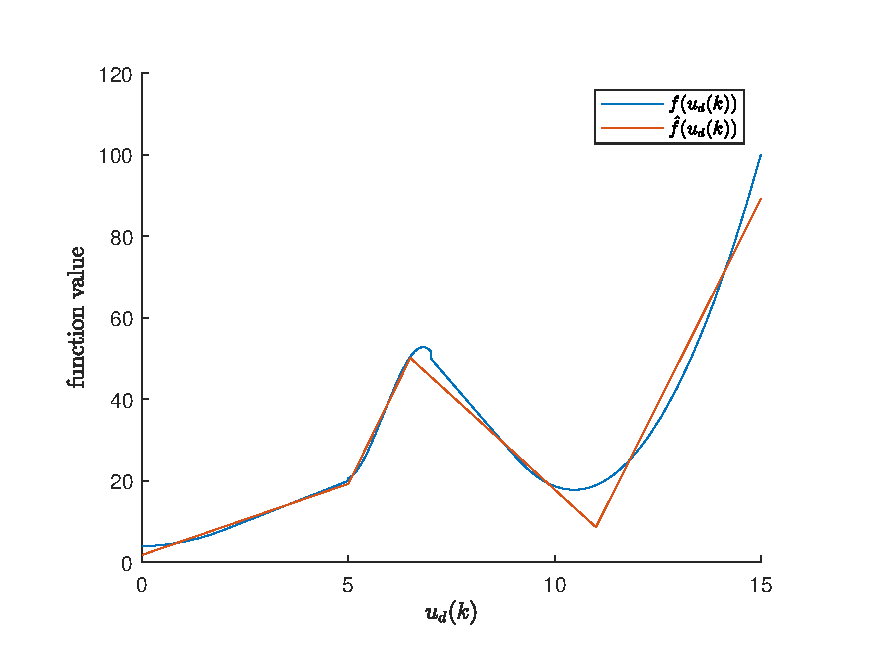
\includegraphics[width=0.8\textwidth]{Latex/images/step23.pdf}
    \caption{AWP approximation comparison}
    \label{fig:part23}
\end{figure}
